% REMEMBER: You must not plagiarise anything in your report. Be extremely careful.
\documentclass{l4proj}

%==============================================================================
% Put any additional packages here
% You can add any packages you want, as long as it does not alter the overall format (e.g. don't change the margins or the reference style).
%
\usepackage{pdfpages} % if you want to include a PDF for an ethics checklist, for example


\begin{document}

%==============================================================================
%% METADATA
\title{Automatic Illustration of Text via Multimodal Interaction}
\author{Stergious Aji (2546916A)}
\date{\today}

\maketitle

%==============================================================================
%% ABSTRACT
\begin{abstract}
    This paper describes a system that automatically illustrates textual information present in audio sources and presents a ground truth builder for automatic videography evaluations.
    
    Users can use this system as a standard automated videography tool that generates videos with relevant imagery appearing in time with the text in the audio. Alternatively, they can build ground truth data for various audio sources. This ground truth would consist of timing information as well as sets of true labelled images for each chunk within the audio.

    
    
    % Every abstract follows a similar pattern. Motivate; set aims; describe work; explain results.
    % \vskip 0.5em
    % ``XYZ is bad. This project investigated ABC to determine if it was better. 
    % ABC used XXX and YYY to implement ZZZ. This is particularly interesting as XXX and YYY have
    % never been used together. It was found that  
    % ABC was 20\% better than XYZ, though it caused rabies in half of subjects.''
\end{abstract}

%==============================================================================
%% ACKNOWLEDGEMENTS
\chapter*{Acknowledgements}
% Enter any acknowledgements here. This is optional; you may leave this blank if you wish, or remove the entire chapter
%
% We give thanks to the Gods of LaTeX, who in their eternal graciousness, have granted that this document may compile without errors or overfull hboxes.

%==============================================================================
% EDUCATION REUSE CONSENT FORM
% If you consent to your project being shown to future students for educational purposes then insert your name and the date below to  sign the education use form that appears in the front of the document. You must explicitly give consent if you wish to do so.
% If you sign, your project may be included in the Hall of Fame if it scores particularly highly.
%
% Please note that you are under no obligation to sign this declaration, but doing so would help future students.

\def\consentname {Stergious Aji} % your full name
\def\consentdate {\today} % the date you agree
\educationalconsent


%==============================================================================
\tableofcontents
%==============================================================================
%% Notes on formatting
%==============================================================================
% The first page, abstract and table of contents are numbered using Roman numerals and are not included in the page count. 
%
% From now on pages are numbered using Arabic numerals. Therefore, immediately after the first call to \chapter we need the call \pagenumbering{arabic} and this should be called once only in the document. 
%
%
% The first Chapter should then be on page 1. 

% PAGE LIMITS
% You are allowed 40 pages for a 40 credit project and 30 pages for a 20 credit report. This includes everything numbered in Arabic numerals (excluding front matter) up to but *excluding the appendices and bibliography*.
%
% FORMATTING
% You must not alter text size (it is currently 10pt) or alter margins or spacing. Do not alter the bibliography style. 
%
%================================================================================
%
% IMPORTANT
% The chapter headings and structure here are **suggestions**. You don't have to follow this model if it doesn't fit your project. Every project should have an introduction and conclusion, however.  If in doubt, your supervisor can give you specific guidance; their view takes precedence over the structure suggested here.
%
%================================================================================
\chapter{Introduction}
% reset page numbering. Don't remove this!
\pagenumbering{arabic} 

% Why should the reader care about what are you doing and what are you actually doing?
This chapter serves to outline the motivations for creating an automatic videography tool, as well as the rationale for a subsequent ground truth builder web application, specifically using multimodal representations of images and text.

% \textbf{Motivate} first, then state the general problem clearly. 
\section{Motivation}
\subsection{Automatic Videography}
Automatic video generation is a broad topic with many applications in today's media-heavy landscape. The rise in video production, both in terms of the number of people making video content and the number of videos being made daily, has motivated more automated systems to aid in this process. This is especially true for music which often has no corresponding video content for many different reasons. For instance, no official music video has been created by the artist due to a lack of funding or song popularity, or the audio track could be digitised from an older format, like vinyl. 

(VIDEO PLATFORMS: YOUTUBE, TIKTOK ETC.)

However, a tool like this could be used for more diverse content such as illustrating educational content and podcasts. Studies (CITE) have shown that users are more engaged and take in more information from multimodal content compared to (unary!) content such as text-only or audio-only. Increased engagement means an improved learning experience as a video can encompass three different modes for the same information, including, visual, auditory, and textual simultaneously. This makes it more accessible to people of different learning lifestyles present in the VARK acronym (CITE).

(IMPROVEMENTS TO ANDREW PARKER'S DISS)

\subsection{Ground Truth Builder}
This increase in media consumption and creation has ultimately caused a rise in automated videography systems. However, we found that there is currently no objective procedure for evaluating comparative performances between different systems. More specifically in measuring their accuracy at image retrieving from  text. Image relevance can and has been measured with qualitative user surveys but this can often be very subjective on personal preferences and (current) moods. More importantly, to evaluate a new system, more user studies must be conducted with the same demographic of people if the end goal is to compare against the results of a previously evaluated system. This is impractical, not to mention, very time-consuming and producing non-repeatable and biased evaluations.

This can be mitigated if instead a set of true labels are made for provided audio sources beforehand which can then be used to evaluate any number of videography systems on those same audio tracks. It is important that the same static image collection is used for ground truth building and evaluating in order to produce repeatable and standardised performance metrics.

This called for a user-friendly interface to build ground truths for a given audio source which, under the hood, can use the same pipeline as the automated videography system that we are creating.

\section{Aims}
This project aims to produce a piece of software that can take any audio source and automatically generate a video from it. The video will consist of relevant imagery corresponding to the textual content present in the audio, as well as, appearing in a timely manner. Additionally, some functionality that lets the user build a ground truth for a given audio source. This will be achieved by letting the user select the set of images that they perceive as the most fitting to the accompanying text or lyric in a given chunk of audio. This set of images will be picked from a top-$k$ which will be retrieved from searching a multimodal space of embedded images and text.

Since there is a high priority for precise ground truth building; the software must be intuitive to use with clear instructions for the user to follow. We must, therefore, aim to produce a user-friendly interface in an easily accessible platform such as a web application. Additionally, since the target demographic is any user willing to create a video. (REWORD WTF) Appropriate error handling must be in place to guide users from a wide area of technical backgrounds.

(MODULARITY OF BACKEND/FRONTEND TO BE USED WITH ANY IMAGE COLLECTION)
We also aim to make our system modular, meaning that ground truths can be made and evaluated with any static image collection the user desires, with very minimal configuring required. 

(FIX FALLBACKS FROM PARKER'S DISS)


%================================================================================
\chapter{Background}
What did other people do, and how is it relevant to what you want to do?
\section{Guidance}
\begin{itemize}    
    \item
      Don't give a laundry list of references.
    \item
      Tie everything you say to your problem.
    \item
      Present an argument.
    \item Think critically; weigh up the contribution of the background and put it in context.    
    \item
      \textbf{Don't write a tutorial}; provide background and cite
      references for further information.
\end{itemize}

%================================================================================
\chapter{Analysis/Requirements}
(USER STORIES?? MOSCOW PRIORITISATION)

This chapter serves to break down the high-level aims of the project in order to produce a list of functional and non-functional requirements, ordered by priority. This will directly determine the design and implementation of the project.

\section{Problems with Previous Thesis}
The previous Automatic Videography system implemented by Andrew Parker (CAN I MENTION NAME?) (CITE) made many achievements in generating complementary videos for audio tracks. However, it was restricted to the YouTube platform and emerged with a number of unforeseen drawbacks. Firstly, the metadata from YouTube was found to be unreliable in obtaining the artist's name and the song title of the song. Therefore, this information was acquired from the user inputting the correct details when using the system. This can be problematic since this requires the user to perform more work of researching and correctly typing in this information which is prone to errors. The previous system also relied on many different Application Programming Interfaces (APIs) like YAKE (CITE) for keyword extraction, and Google Images Search (CITE) to download the images. This places high 


What is the problem that you want to solve, and how did you arrive at it?
\section{Guidance}
Make it clear how you derived the constrained form of your problem via a clear and logical process. 

The analysis chapter explains the process by which you arrive at a concrete design. In software 
engineering projects, this will include a statement of the requirement capture process and the
derived requirements.

In research projects, it will involve developing a design drawing on
the work established in the background, and stating how the space of possible projects was
sensibly narrowed down to what you have done.

%================================================================================
\chapter{Design}
How is this problem to be approached, without reference to specific implementation details? 
\section{Guidance}
Design should cover the abstract design in such a way that someone else might be able to do what you did, 
but with a different language or library or tool. This might include overall system architecture diagrams,
user interface designs (wireframes/personas/etc.), protocol specifications, algorithms, data set design choices,
among others. Specific languages, technical choices, libraries and such like should not usually appear in the design. These are implementation details.


%================================================================================
\chapter{Implementation}
What did you do to implement this idea, and what technical achievements did you make?
\section{Guidance}
You can't talk about everything. Cover the high level first, then cover important, relevant or impressive details.

\section{General guidance for technical writing}

These points apply to the whole dissertation, not just this chapter.

\subsection{Figures}
\emph{Always} refer to figures included, like Figure \ref{fig:relu}, in the body of the text. Include full, explanatory captions and make sure the figures look good on the page.
You may include multiple figures in one float, as in Figure \ref{fig:synthetic}, using \texttt{subcaption}, which is enabled in the template.


% Figures are important. Use them well.
\begin{figure}[htb]
    \centering
    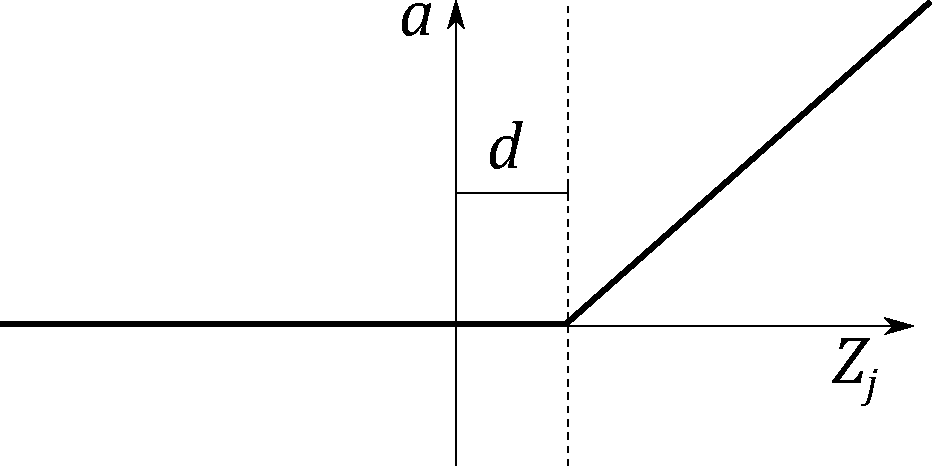
\includegraphics[width=0.5\linewidth]{images/relu.pdf}    

    \caption{In figure captions, explain what the reader is looking at: ``A schematic of the rectifying linear unit, where $a$ is the output amplitude,
    $d$ is a configurable dead-zone, and $Z_j$ is the input signal'', as well as why the reader is looking at this: 
    ``It is notable that there is no activation \emph{at all} below 0, which explains our initial results.'' 
    \textbf{Use vector image formats (.pdf) where possible}. Size figures appropriately, and do not make them over-large or too small to read.
    }

    % use the notation fig:name to cross reference a figure
    \label{fig:relu} 
\end{figure}


\begin{figure}[htb] 
    \centering
    \begin{subfigure}[b]{0.45\textwidth}
        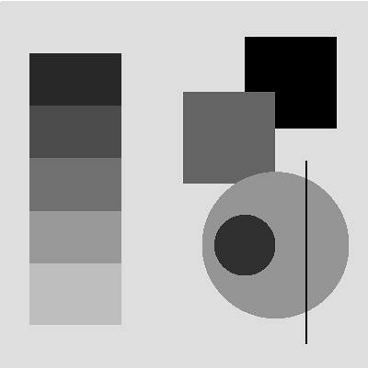
\includegraphics[width=\textwidth]{images/synthetic.png}
        \caption{Synthetic image, black on white.}
        \label{fig:syn1}
    \end{subfigure}
    ~ %add desired spacing between images, e. g. ~, \quad, \qquad, \hfill etc. 
      %(or a blank line to force the subfigure onto a new line)
    \begin{subfigure}[b]{0.45\textwidth}
        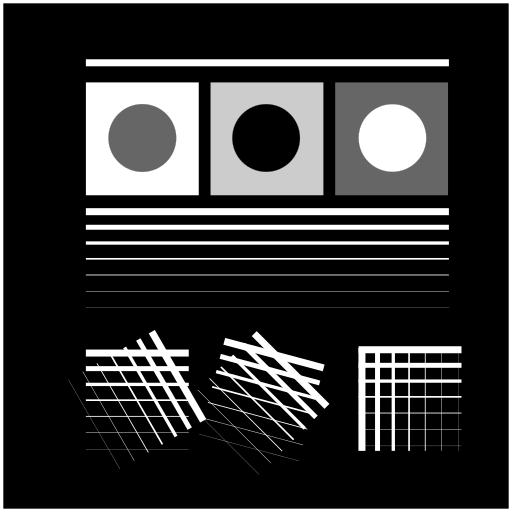
\includegraphics[width=\textwidth]{images/synthetic_2.png}
        \caption{Synthetic image, white on black.}
        \label{fig:syn2}
    \end{subfigure}
    ~ %add desired spacing between images, e. g. ~, \quad, \qquad, \hfill etc. 
    %(or a blank line to force the subfigure onto a new line)    
    \caption{Synthetic test images for edge detection algorithms. \subref{fig:syn1} shows various gray levels that require an adaptive algorithm. \subref{fig:syn2}
    shows more challenging edge detection tests that have crossing lines. Fusing these into full segments typically requires algorithms like the Hough transform.
    This is an example of using subfigures, with \texttt{subref}s in the caption.
    }\label{fig:synthetic}
\end{figure}

\clearpage

\subsection{Equations}

Equations should be typeset correctly and precisely. Make sure you get parenthesis sizing correct, and punctuate equations correctly 
(the comma is important and goes \textit{inside} the equation block). Explain any symbols used clearly if not defined earlier. 

For example, we might define:
\begin{equation}
    \hat{f}(\xi) = \frac{1}{2}\left[ \int_{-\infty}^{\infty} f(x) e^{2\pi i x \xi} \right],
\end{equation}    
where $\hat{f}(\xi)$ is the Fourier transform of the time domain signal $f(x)$.

\subsection{Algorithms}
Algorithms can be set using \texttt{algorithm2e}, as in Algorithm \ref{alg:metropolis}.

% NOTE: line ends are denoted by \; in algorithm2e
\begin{algorithm}
    \DontPrintSemicolon
    \KwData{$f_X(x)$, a probability density function returing the density at $x$.\; $\sigma$ a standard deviation specifying the spread of the proposal distribution.\;
    $x_0$, an initial starting condition.}
    \KwResult{$s=[x_1, x_2, \dots, x_n]$, $n$ samples approximately drawn from a distribution with PDF $f_X(x)$.}
    \Begin{
        $s \longleftarrow []$\;
        $p \longleftarrow f_X(x)$\;
        $i \longleftarrow 0$\;
        \While{$i < n$}
        {
            $x^\prime \longleftarrow \mathcal{N}(x, \sigma^2)$\;
            $p^\prime \longleftarrow f_X(x^\prime)$\;
            $a \longleftarrow \frac{p^\prime}{p}$\;
            $r \longleftarrow U(0,1)$\;
            \If{$r<a$}
            {
                $x \longleftarrow x^\prime$\;
                $p \longleftarrow f_X(x)$\;
                $i \longleftarrow i+1$\;
                append $x$ to $s$\;
            }
        }
    }
    
\caption{The Metropolis-Hastings MCMC algorithm for drawing samples from arbitrary probability distributions, 
specialised for normal proposal distributions $q(x^\prime|x) = \mathcal{N}(x, \sigma^2)$. The symmetry of the normal distribution means the acceptance rule takes the simplified form.}\label{alg:metropolis}
\end{algorithm}

\subsection{Tables}

If you need to include tables, like Table \ref{tab:operators}, use a tool like https://www.tablesgenerator.com/ to generate the table as it is
extremely tedious otherwise. 

\begin{table}[]
    \caption{The standard table of operators in Python, along with their functional equivalents from the \texttt{operator} package. Note that table
    captions go above the table, not below. Do not add additional rules/lines to tables. }\label{tab:operators}
    %\tt 
    \rowcolors{2}{}{gray!3}
    \begin{tabular}{@{}lll@{}}
    %\toprule
    \textbf{Operation}    & \textbf{Syntax}                & \textbf{Function}                            \\ %\midrule % optional rule for header
    Addition              & \texttt{a + b}                          & \texttt{add(a, b)}                                    \\
    Concatenation         & \texttt{seq1 + seq2}                    & \texttt{concat(seq1, seq2)}                           \\
    Containment Test      & \texttt{obj in seq}                     & \texttt{contains(seq, obj)}                           \\
    Division              & \texttt{a / b}                          & \texttt{div(a, b) }  \\
    Division              & \texttt{a / b}                          & \texttt{truediv(a, b) } \\
    Division              & \texttt{a // b}                         & \texttt{floordiv(a, b)}                               \\
    Bitwise And           & \texttt{a \& b}                         & \texttt{and\_(a, b)}                                  \\
    Bitwise Exclusive Or  & \texttt{a \textasciicircum b}           & \texttt{xor(a, b)}                                    \\
    Bitwise Inversion     & \texttt{$\sim$a}                        & \texttt{invert(a)}                                    \\
    Bitwise Or            & \texttt{a | b}                          & \texttt{or\_(a, b)}                                   \\
    Exponentiation        & \texttt{a ** b}                         & \texttt{pow(a, b)}                                    \\
    Identity              & \texttt{a is b}                         & \texttt{is\_(a, b)}                                   \\
    Identity              & \texttt{a is not b}                     & \texttt{is\_not(a, b)}                                \\
    Indexed Assignment    & \texttt{obj{[}k{]} = v}                 & \texttt{setitem(obj, k, v)}                           \\
    Indexed Deletion      & \texttt{del obj{[}k{]}}                 & \texttt{delitem(obj, k)}                              \\
    Indexing              & \texttt{obj{[}k{]}}                     & \texttt{getitem(obj, k)}                              \\
    Left Shift            & \texttt{a \textless{}\textless b}       & \texttt{lshift(a, b)}                                 \\
    Modulo                & \texttt{a \% b}                         & \texttt{mod(a, b)}                                    \\
    Multiplication        & \texttt{a * b}                          & \texttt{mul(a, b)}                                    \\
    Negation (Arithmetic) & \texttt{- a}                            & \texttt{neg(a)}                                       \\
    Negation (Logical)    & \texttt{not a}                          & \texttt{not\_(a)}                                     \\
    Positive              & \texttt{+ a}                            & \texttt{pos(a)}                                       \\
    Right Shift           & \texttt{a \textgreater{}\textgreater b} & \texttt{rshift(a, b)}                                 \\
    Sequence Repetition   & \texttt{seq * i}                        & \texttt{repeat(seq, i)}                               \\
    Slice Assignment      & \texttt{seq{[}i:j{]} = values}          & \texttt{setitem(seq, slice(i, j), values)}            \\
    Slice Deletion        & \texttt{del seq{[}i:j{]}}               & \texttt{delitem(seq, slice(i, j))}                    \\
    Slicing               & \texttt{seq{[}i:j{]}}                   & \texttt{getitem(seq, slice(i, j))}                    \\
    String Formatting     & \texttt{s \% obj}                       & \texttt{mod(s, obj)}                                  \\
    Subtraction           & \texttt{a - b}                          & \texttt{sub(a, b)}                                    \\
    Truth Test            & \texttt{obj}                            & \texttt{truth(obj)}                                   \\
    Ordering              & \texttt{a \textless b}                  & \texttt{lt(a, b)}                                     \\
    Ordering              & \texttt{a \textless{}= b}               & \texttt{le(a, b)}                                     \\
    % \bottomrule
    \end{tabular}
    \end{table}
\subsection{Code}

Avoid putting large blocks of code in the report (more than a page in one block, for example). Use syntax highlighting if possible, as in Listing \ref{lst:callahan}.

\begin{lstlisting}[language=python, float, caption={The algorithm for packing the $3\times 3$ outer-totalistic binary CA successor rule into a 
    $16\times 16\times 16\times 16$ 4 bit lookup table, running an equivalent, notionally 16-state $2\times 2$ CA.}, label=lst:callahan]
    def create_callahan_table(rule="b3s23"):
        """Generate the lookup table for the cells."""        
        s_table = np.zeros((16, 16, 16, 16), dtype=np.uint8)
        birth, survive = parse_rule(rule)

        # generate all 16 bit strings
        for iv in range(65536):
            bv = [(iv >> z) & 1 for z in range(16)]
            a, b, c, d, e, f, g, h, i, j, k, l, m, n, o, p = bv

            # compute next state of the inner 2x2
            nw = apply_rule(f, a, b, c, e, g, i, j, k)
            ne = apply_rule(g, b, c, d, f, h, j, k, l)
            sw = apply_rule(j, e, f, g, i, k, m, n, o)
            se = apply_rule(k, f, g, h, j, l, n, o, p)

            # compute the index of this 4x4
            nw_code = a | (b << 1) | (e << 2) | (f << 3)
            ne_code = c | (d << 1) | (g << 2) | (h << 3)
            sw_code = i | (j << 1) | (m << 2) | (n << 3)
            se_code = k | (l << 1) | (o << 2) | (p << 3)

            # compute the state for the 2x2
            next_code = nw | (ne << 1) | (sw << 2) | (se << 3)

            # get the 4x4 index, and write into the table
            s_table[nw_code, ne_code, sw_code, se_code] = next_code

        return s_table

\end{lstlisting}

%==================================================================================================================================
\chapter{Evaluation} 
How good is your solution? How well did you solve the general problem, and what evidence do you have to support that?

\section{Guidance}
\begin{itemize}
    \item
        Ask specific questions that address the general problem.
    \item
        Answer them with precise evidence (graphs, numbers, statistical
        analysis, qualitative analysis).
    \item
        Be fair and be scientific.
    \item
        The key thing is to show that you know how to evaluate your work, not
        that your work is the most amazing product ever.
\end{itemize}

\section{Evidence}
Make sure you present your evidence well. Use appropriate visualisations, 
reporting techniques and statistical analysis, as appropriate. The point is not
to dump all the data you have but to present an argument well supported by evidence gathered.

If you use numerical evidence, specify reasonable numbers of significant digits; don't state ``18.41141\% of users were successful'' if you only had 20 users. If you average \textit{anything}, present both a measure of central tendency (e.g. mean, median) \textit{and} a measure of spread (e.g. standard deviation, min/max, interquartile range).

You can use \texttt{siunitx} to define units, space numbers neatly, and set the precision for the whole LaTeX document. 

% setup siunitx to have two decimal places
\sisetup{
	round-mode = places,
	round-precision = 2
}

For example, these numbers will appear with two decimal places: \num{3.141592}, \num{2.71828}, and this one will appear with reasonable spacing \num{1000000}.



If you use statistical procedures, make sure you understand the process you are using,
and that you check the required assumptions hold in your case. 

If you visualise, follow the basic rules, as illustrated in Figure \ref{fig:boxplot}:
\begin{itemize}
\item Label everything correctly (axis, title, units).
\item Caption thoroughly.
\item Reference in text.
\item \textbf{Include appropriate display of uncertainty (e.g. error bars, Box plot)}
\item Minimize clutter.
\end{itemize}

See the file \texttt{guide\_to\_visualising.pdf} for further information and guidance.

\begin{figure}[htb]
    \centering
    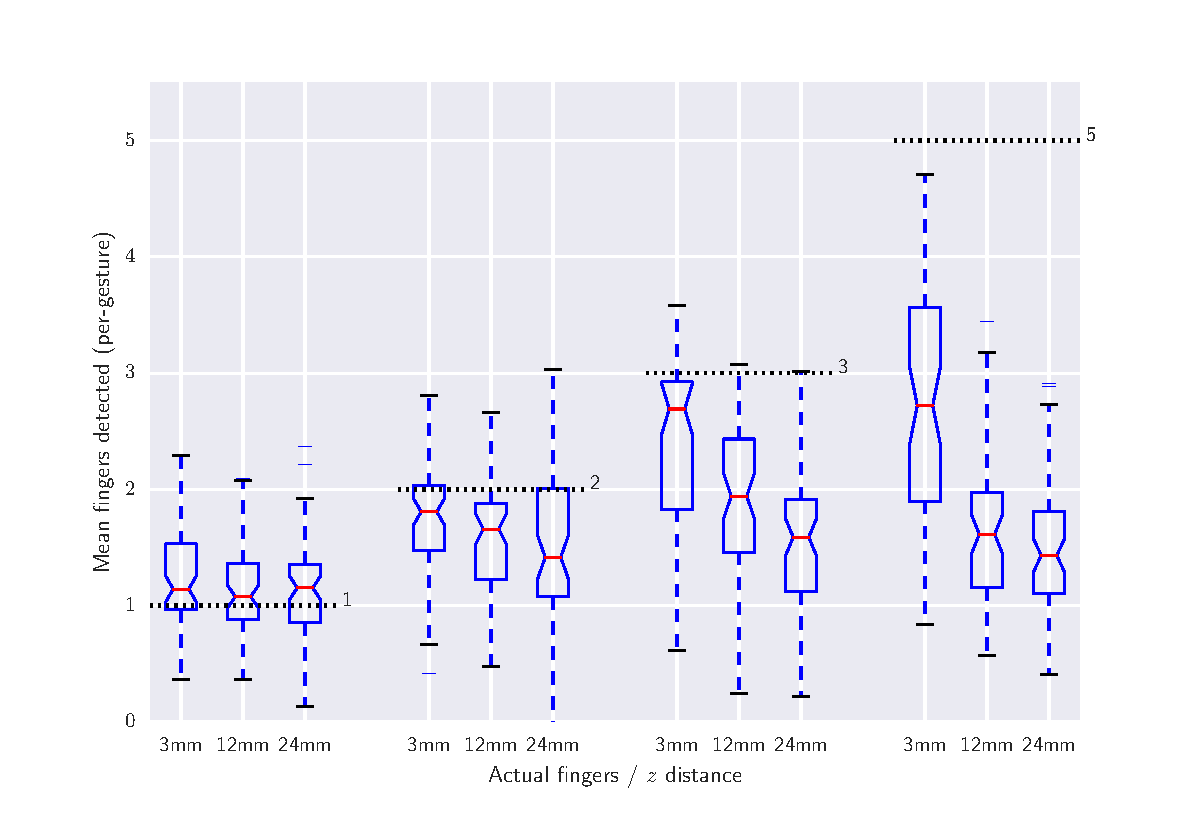
\includegraphics[width=1.0\linewidth]{images/boxplot_finger_distance.pdf}    

    \caption{Average number of fingers detected by the touch sensor at different heights above the surface, averaged over all gestures. Dashed lines indicate
    the true number of fingers present. The Box plots include bootstrapped uncertainty notches for the median. It is clear that the device is biased toward 
    undercounting fingers, particularly at higher $z$ distances.
    }

    % use the notation fig:name to cross reference a figure
    \label{fig:boxplot} 
\end{figure}


%==================================================================================================================================
\chapter{Conclusion}    
Summarise the whole project for a lazy reader who didn't read the rest (e.g. a prize-awarding committee). This chapter should be short in most dissertations; maybe one to three pages.
\section{Guidance}
\begin{itemize}
    \item
        Summarise briefly and fairly.
    \item
        You should be addressing the general problem you introduced in the
        Introduction.        
    \item
        Include summary of concrete results (``the new compiler ran 2x
        faster'')
    \item
        Indicate what future work could be done, but remember: \textbf{you
        won't get credit for things you haven't done}.
\end{itemize}

\section{Summary}
Summarise what you did; answer the general questions you asked in the introduction. What did you achieve? Briefly describe what was built and summarise the evaluation results.

\section{Reflection}
Discuss what went well and what didn't and how you would do things differently if you did this project again.

\section{Future work}
Discuss what you would do if you could take this further -- where would the interesting directions to go next be? (e.g. you got another year to work on it, or you started a company to work on this, or you pursued a PhD on this topic)

%==================================================================================================================================
%
% 
%==================================================================================================================================
%  APPENDICES  

\begin{appendices}

\chapter{Appendices}
 (ETHICS CHECKLIST + INTRODUCTION BRIEF)
 
Use separate appendix chapters for groups of ancillary material that support your dissertation. 
Typical inclusions in the appendices are:

\begin{itemize}
\item
  Copies of ethics approvals (you must include these if you needed to get them)
\item
  Copies of questionnaires etc. used to gather data from subjects. Don't include
  voluminous data logs; instead submit these electronically alongside your source code.
\item
  Extensive tables or figures that are too bulky to fit in the main body of
  the report, particularly ones that are repetitive and summarised in the body.
\item Outline of the source code (e.g. directory structure), 
    or other architecture documentation like class diagrams.
\item User manuals, and any guides to starting/running the software. 
Your equivalent of \texttt{readme.md} should be included.

\end{itemize}

\textbf{Don't include your source code in the appendices}. It will be
submitted separately.



\end{appendices}

%==================================================================================================================================
%   BIBLIOGRAPHY   

% The bibliography style is agsm (Harvard)
% The bibliography always appears last, after the appendices.

\bibliographystyle{agsm}

% Force the bibliography not to be numbered
\renewcommand{\thechapter}{0} 
\bibliography{l4proj}

\end{document}
